% File name: datalogger/Reports/Final_Report_Andy.tex
% Final report for datalogger project
% Author: adh
% Date: Mon 03 Jun 2013 11:51

\documentclass[a4paper,10pt]{article}  % Standard document class
\usepackage[english]{babel}            % Set document language
\usepackage{fullpage}                  % Set up page for small margins etc

\usepackage{graphicx}                  % For including images in document
\usepackage{placeins}                  % Allows use of \FloatBarrier
% to avoid images or tables
% moving into next section
\usepackage{subfig}                    % For subfigures...

\usepackage{amsmath}                   % For improving maths/formula typesetting
\usepackage{tabularx}                  % Table changing package

\usepackage{algpseudocode}             % For producing algorithms/flowcharts
\usepackage{listings}                  % For including source code in document

\usepackage{url}

% Provide command for scientific notation
\providecommand{\e}[1]{\ensuremath{\times10^{#1}}}
\providecommand{\degrees}{\ensuremath{^{\circ}}}

% Define title here:
\title{Project SB3: Data Logger\\
       Package Environment Monitoring\\
       Final Report}
\author{Andrew Holt\\
        ah635\\
        Team 6\\
        Emmanuel}
\date{06 June 2013}

\begin{document}

% generate title
\maketitle

\begin{center}
  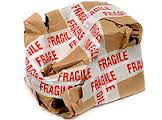
\includegraphics[width=0.3\textwidth]{damaged_parcel.jpg}
\end{center}

\noindent summary: motive, method, key results, conclusions

\tableofcontents

\section{Introduction}
\label{sec:introduction}

The express delivery industry is one of the fastest growing industries
in the world today. In 2003, the industry made a direct contribution
of US\$64 billion to worldwide GDP, and has been growing by around 8\%
per year since \cite{OEF2005}. However, customers have very little
information of the environmental and handling conditions their package
has been subject to during its transit. When shipping fragile or
sensitive products, the conditions that the parcel is subject to may
be critical in the integrity of the product. The two major issues here
are:
\begin{enumerate}
\item Fragile goods which arrive broken: it is desirable to determine
  whether the package has been mishandled, and if so by whom.
\item Perishable goods: if they have been subjected to conditions
  outside of temperature and humidity sensitive limits they will have
  a shorted shelf life. This may not be obvious upon inspection of the
  goods, so detailed condition tracking is required.
\end{enumerate}
While products have been around for a while to carry out this type of
tracking on shipping containers, the same problem applies to smaller
and domestic packages too. In the past six months, a couple of
products have been announced to achieve this, but it is clearly an
emerging market and a good product launched now could have a great
chance of success. FedEx Corporation have recently announced
deployment of a similar environmental tracking device,
``SenseAware''\cite{SA_PR}, however this is only available on a select
number of carriers and services and is a business level product, not
suited for everyday or relatively low value package monitoring. An
alternative is the ``DropTag'' system recently announced by Cambridge
Consultants \cite{DT_PR}, however this system is not yet at the
commercial release stage.

With a problem identified and a solution required, as well as a clear
business opportunity due to the interest in development from other
companies, product development was begun.

\section{Overview}
\label{sec:overview}

In order to effectively track the condition of a parcel during
transit, the final product was clearly required to be cheap, low power
and physically small and robust. For this project, a simple prototype
was to be developed, which if successful could be miniaturised and
fabricated for the final product.

\subsection{Summary of Design}
\label{sec:summary-design}

The first stage of the design process was to evaluate which quantities
should be measured and logged. The key environmental variables would
be temperature and humidity. Vibration, orientation and shocks would
also be required to understand the handling and transport
conditions. GPS tracking would also be useful, but it was decided to
focus on the other five initially as GPS could be relatively simply
included with a dedicated GPS chip communicating over the I$^2$C
protocol, and GPS reception may be limited at many points during
transit.

The product would clearly be required to work without being plugged in
to a computer, so a standalone mode would be developed. It would be
useful for development, debugging and testing to operate with instant
feedback from the computer system, so a linked mode was also
developed.

To ensure long term operation, on-board memory would be required, so an
EEPROM was used for data storage in the standalone mode. This would
also require a battery supply.

Some kind of on-board display would also be useful on the board, for
monitoring, debugging and status display, so an LCD screen was used
along with five LEDs.

The platform choices were specified in the project requirements, so
the project was to be developed for the STM32F100 ARM Cortex MCU and a
PC running the Windows operating system. The key design areas would
therefore be hardware, firmware and software. The budget was generous
for the development board so cost was not really an issue, however to
achieve a commercial product, the cost and size would need to be
reduced. This could be achieved by miniaturising, as surface mount
components tend to be cheaper, use of a cheaper MCU (which wouldn't
need the development features of the STM).

The project block diagram is shown in figure \ref{fig:sysblkdgrm}.
\begin{figure}[htb]
  \begin{center}
    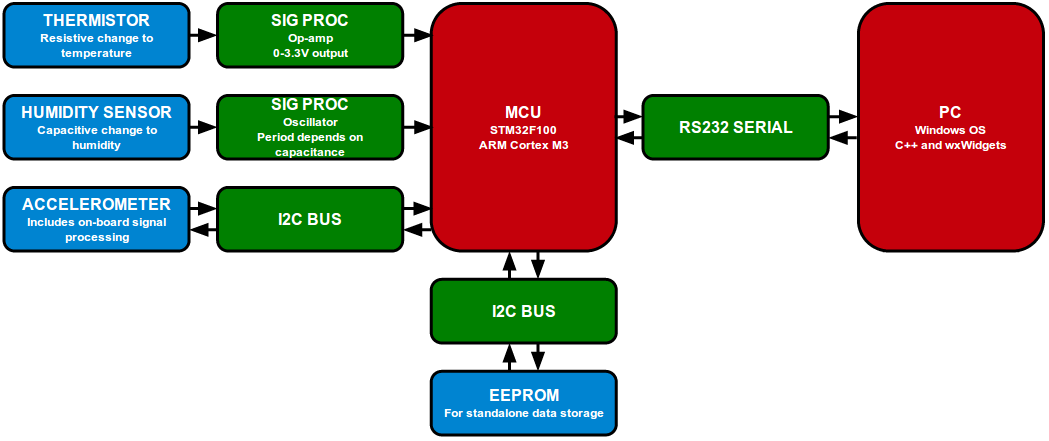
\includegraphics[width=1.0\textwidth]{System_diagram.png}
  \end{center}
  \caption{Overall system block diagram}
  \label{fig:sysblkdgrm}
\end{figure}

\subsection{Project Management}
\label{sec:project-management}

The project was divided between the two team members. It was decided
that James would write the firmware for the MCU, Andrew would write
the software for the computer and the hardware design was to be
shared. The general development plan was to start by making a basic
but working system and gradually adding features and complexity upon
the existing system. This ensured that we would have a fully
operational, if not with every desired feature, by the end of the
project, and would also allow the simpler parts to be used in testing
more complex parts.

Initally basic hardware circuits were designed and built. The firmware
and software were then developed. The hardware circuits were highly
useful in testing the firmware, but in writing the firmware, flaws in
the circuit designs became apparent, such as the initial plan to use a
simple charge-discharge of the humidity sensor. For this reason, the
humidity sensor circuit was updated during the project.

\section{Design}
\label{sec:design}

A brief overview of the design has been given in section
\ref{sec:summary-design}. This section gives technical detail about
the parts of the system which I designed. The other parts are detailed
in James' report.

\subsection{Hardware}
\label{sec:hardware}



\subsection{Software}
\label{sec:software}

\subsection{Communications}

\section{Problems Encountered and Technical Solutions}
\label{sec:probl-enco-techn}

\section{Test Procedures}
\label{sec:test-procedures}

\section{Conclusions and Next Steps}
\label{sec:concl-next-steps}

\appendix

\section{Source Code and Circuit Diagrams}
\label{sec:source-code-circuit}

\section{Marketing Datasheet}
\label{sec:marketing-datasheet}

\section{First Interim Report}
\label{sec:first-interim-report}

\bibliographystyle{plain}
\bibliography{Final_Report_Andy}

\end{document}
